% Created by tikzDevice version 0.7.0 on 2015-04-30 10:54:44
% !TEX encoding = UTF-8 Unicode
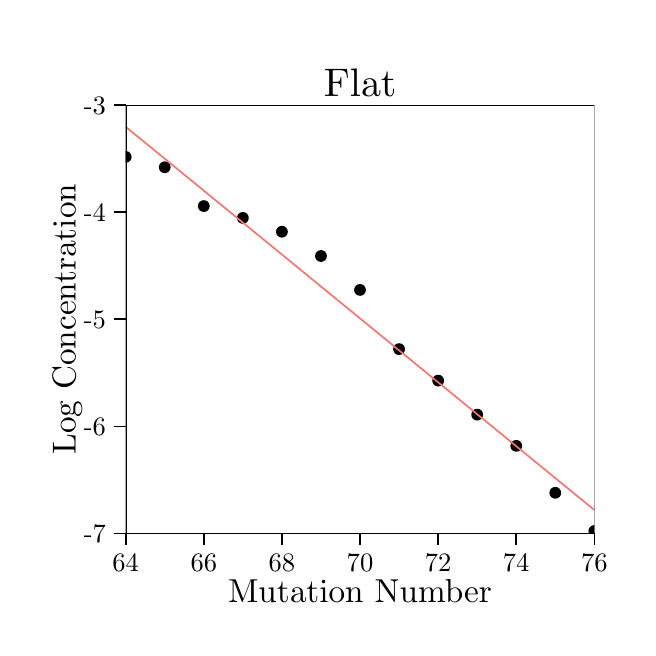
\begin{tikzpicture}[x=1pt,y=1pt]
\definecolor[named]{fillColor}{rgb}{1.00,1.00,1.00}
\path[use as bounding box,fill=fillColor,fill opacity=0.00] (0,0) rectangle (216.81,216.81);
\begin{scope}
\path[clip] (  0.00,  0.00) rectangle (216.81,216.81);
\definecolor[named]{drawColor}{rgb}{1.00,1.00,1.00}
\definecolor[named]{fillColor}{rgb}{1.00,1.00,1.00}

\path[draw=drawColor,line width= 0.6pt,line join=round,line cap=round,fill=fillColor] (  0.00,  0.00) rectangle (216.81,216.81);
\end{scope}
\begin{scope}
\path[clip] ( 35.42, 34.03) rectangle (204.76,188.82);
\definecolor[named]{fillColor}{rgb}{1.00,1.00,1.00}

\path[fill=fillColor] ( 35.42, 34.03) rectangle (204.76,188.82);
\definecolor[named]{fillColor}{rgb}{0.00,0.00,0.00}

\path[fill=fillColor] ( 35.42,170.11) circle (  2.13);

\path[fill=fillColor] ( 49.53,166.37) circle (  2.13);

\path[fill=fillColor] ( 63.64,152.35) circle (  2.13);

\path[fill=fillColor] ( 77.76,148.07) circle (  2.13);

\path[fill=fillColor] ( 91.87,143.08) circle (  2.13);

\path[fill=fillColor] (105.98,134.30) circle (  2.13);

\path[fill=fillColor] (120.09,122.05) circle (  2.13);

\path[fill=fillColor] (134.20,100.65) circle (  2.13);

\path[fill=fillColor] (148.32, 89.27) circle (  2.13);

\path[fill=fillColor] (162.43, 76.98) circle (  2.13);

\path[fill=fillColor] (176.54, 65.70) circle (  2.13);

\path[fill=fillColor] (190.65, 48.74) circle (  2.13);

\path[fill=fillColor] (204.76, 34.93) circle (  2.13);
\definecolor[named]{drawColor}{rgb}{0.97,0.46,0.43}
\definecolor[named]{fillColor}{rgb}{0.97,0.46,0.43}

\path[draw=drawColor,line width= 0.6pt,line join=round,fill=fillColor] ( 35.42,180.98) -- (204.76, 42.50);
\definecolor[named]{drawColor}{rgb}{0.00,0.00,0.00}

\path[draw=drawColor,line width= 0.6pt,line join=round,line cap=round] ( 35.42, 34.03) rectangle (204.76,188.82);
\end{scope}
\begin{scope}
\path[clip] (  0.00,  0.00) rectangle (216.81,216.81);
\definecolor[named]{drawColor}{rgb}{0.00,0.00,0.00}

\node[text=drawColor,anchor=base east,inner sep=0pt, outer sep=0pt, scale=  0.96] at ( 28.31, 30.73) {-7};

\node[text=drawColor,anchor=base east,inner sep=0pt, outer sep=0pt, scale=  0.96] at ( 28.31, 69.43) {-6};

\node[text=drawColor,anchor=base east,inner sep=0pt, outer sep=0pt, scale=  0.96] at ( 28.31,108.12) {-5};

\node[text=drawColor,anchor=base east,inner sep=0pt, outer sep=0pt, scale=  0.96] at ( 28.31,146.82) {-4};

\node[text=drawColor,anchor=base east,inner sep=0pt, outer sep=0pt, scale=  0.96] at ( 28.31,185.52) {-3};
\end{scope}
\begin{scope}
\path[clip] (  0.00,  0.00) rectangle (216.81,216.81);
\definecolor[named]{drawColor}{rgb}{0.00,0.00,0.00}

\path[draw=drawColor,line width= 0.6pt,line join=round] ( 31.15, 34.03) --
	( 35.42, 34.03);

\path[draw=drawColor,line width= 0.6pt,line join=round] ( 31.15, 72.73) --
	( 35.42, 72.73);

\path[draw=drawColor,line width= 0.6pt,line join=round] ( 31.15,111.43) --
	( 35.42,111.43);

\path[draw=drawColor,line width= 0.6pt,line join=round] ( 31.15,150.13) --
	( 35.42,150.13);

\path[draw=drawColor,line width= 0.6pt,line join=round] ( 31.15,188.82) --
	( 35.42,188.82);
\end{scope}
\begin{scope}
\path[clip] (  0.00,  0.00) rectangle (216.81,216.81);
\definecolor[named]{drawColor}{rgb}{0.00,0.00,0.00}

\path[draw=drawColor,line width= 0.6pt,line join=round] ( 35.42, 29.77) --
	( 35.42, 34.03);

\path[draw=drawColor,line width= 0.6pt,line join=round] ( 63.64, 29.77) --
	( 63.64, 34.03);

\path[draw=drawColor,line width= 0.6pt,line join=round] ( 91.87, 29.77) --
	( 91.87, 34.03);

\path[draw=drawColor,line width= 0.6pt,line join=round] (120.09, 29.77) --
	(120.09, 34.03);

\path[draw=drawColor,line width= 0.6pt,line join=round] (148.32, 29.77) --
	(148.32, 34.03);

\path[draw=drawColor,line width= 0.6pt,line join=round] (176.54, 29.77) --
	(176.54, 34.03);

\path[draw=drawColor,line width= 0.6pt,line join=round] (204.76, 29.77) --
	(204.76, 34.03);
\end{scope}
\begin{scope}
\path[clip] (  0.00,  0.00) rectangle (216.81,216.81);
\definecolor[named]{drawColor}{rgb}{0.00,0.00,0.00}

\node[text=drawColor,anchor=base,inner sep=0pt, outer sep=0pt, scale=  0.96] at ( 35.42, 20.31) {64};

\node[text=drawColor,anchor=base,inner sep=0pt, outer sep=0pt, scale=  0.96] at ( 63.64, 20.31) {66};

\node[text=drawColor,anchor=base,inner sep=0pt, outer sep=0pt, scale=  0.96] at ( 91.87, 20.31) {68};

\node[text=drawColor,anchor=base,inner sep=0pt, outer sep=0pt, scale=  0.96] at (120.09, 20.31) {70};

\node[text=drawColor,anchor=base,inner sep=0pt, outer sep=0pt, scale=  0.96] at (148.32, 20.31) {72};

\node[text=drawColor,anchor=base,inner sep=0pt, outer sep=0pt, scale=  0.96] at (176.54, 20.31) {74};

\node[text=drawColor,anchor=base,inner sep=0pt, outer sep=0pt, scale=  0.96] at (204.76, 20.31) {76};
\end{scope}
\begin{scope}
\path[clip] (  0.00,  0.00) rectangle (216.81,216.81);
\definecolor[named]{drawColor}{rgb}{0.00,0.00,0.00}

\node[text=drawColor,anchor=base,inner sep=0pt, outer sep=0pt, scale=  1.20] at (120.09,  9.03) {Mutation Number};
\end{scope}
\begin{scope}
\path[clip] (  0.00,  0.00) rectangle (216.81,216.81);
\definecolor[named]{drawColor}{rgb}{0.00,0.00,0.00}

\node[text=drawColor,rotate= 90.00,anchor=base,inner sep=0pt, outer sep=0pt, scale=  1.20] at ( 17.30,111.43) {Log Concentration};
\end{scope}
\begin{scope}
\path[clip] (  0.00,  0.00) rectangle (216.81,216.81);
\definecolor[named]{drawColor}{rgb}{0.00,0.00,0.00}

\node[text=drawColor,anchor=base,inner sep=0pt, outer sep=0pt, scale=  1.44] at (120.09,191.84) {Flat};
\end{scope}
\end{tikzpicture}
